%%%%%%%%%%%%%%%%%%%%%%%%%%%%%%%%%%%%%%%%%%%%%%%%
%% Intro to LaTeX and Template for Homework Assignments
%% Quantitative Methods in Political Science
%% University of Mannheim
%% Fall 2017
%%%%%%%%%%%%%%%%%%%%%%%%%%%%%%%%%%%%%%%%%%%%%%%%

% created by Marcel Neunhoeffer & Sebastian Sternberg


% This template and tutorial will help you to write up your homework. It will also help you to use Latex for other assignments than this course's homework.

%%%%%%%%%%%%%%%%%%%%%%%%%%%%%%%%%%%%%%%%%%%%%%%%
% Before we get started
%%%%%%%%%%%%%%%%%%%%%%%%%%%%%%%%%%%%%%%%%%%%%%%%

% Make an account on overleaf.com and get started. No need to install anything.

%%%%%%%%%%%%%%%%%%%%%%%%%%%%%%%%%%%%%%%%%%%%%%%%
% Or if you want it the nerdy way...
% INSTALL LATEX: Before we can get started you need to install LaTeX on your computer.
				% Windows: http://miktex.org/download
				% Mac:         http://www.tug.org/mactex/mactex-download.html	
				% There a many more different LaTeX editors out there for both operating systems. I use TeXworks because it looks the same on Windows and Mac.
				

% SAVE THE FILE: The first thing you need to do is to save your LaTeX file in a directory as a .tex file. You will not be able to do anything else unless your file is saved. I suggest to save the .tex file in the same folder with your .R script and where you will save your plots from R to. Let's call this file template_homework1.tex and save it in your Week 1 folder.


% COMPILE THE FILE: After setting up your file, using your LaTeX editor (texmaker, texshop), you can compile your document using PDFLaTeX.
	% Compiling your file tells LaTeX to take the code you have written and create a pdf file
	% After compiling your file, in your directory will appear four new files, including a .pdf file. This is your output document.
	% It is good to compile your file regularly so that you can see how your code is translating into your document.
	
	
% ERRORS: If you get an error message, something is wrong in your code. Fix errors before they pile up!
	% As with error messages in R, google the exact error message if you have a question!
%%%%%%%%%%%%%%%%%%%%%%%%%%%%%%%%%%%%%%%%%%%%%%%%


% Now again for everyone...

% COMMANDS: 
	% To do anything in LaTeX, you must use commands
	% Commands tell LaTeX when to start your document, how you want your document to look, and how to format your document
	% Commands ALWAYS begin with a backslash \

% Everything following the % sign is a comment and will not be used by Latex to compile your document.
% This is very similar to # comments in R.

% Every .tex file usually consists of four parts.
% 1. Document Class
% 2. Packages
% 3. Header
% 4. Your Document

%%%%%%%%%%%%%%%%%%%%%%%%%%%%%%%%%%%%%%%%%%%%%%%%
% 1. Document Class
%%%%%%%%%%%%%%%%%%%%%%%%%%%%%%%%%%%%%%%%%%%%%%%%
 
 % The first command you will always have will declare your document class. This tells LaTeX what type of document you are creating (article, presentation, poster, etc). 
% \documentclass is the command
% in {} you specify the type of document
% in [] you define additional parameters
 
\documentclass[a4paper,12pt]{article} % This defines the style of your paper

% We usually use the article type. The additional parameters are the format of the paper you want to print it on and the standard font size. For us this is a4paper and 12pt.

%%%%%%%%%%%%%%%%%%%%%%%%%%%%%%%%%%%%%%%%%%%%%%%%
% 2. Packages
%%%%%%%%%%%%%%%%%%%%%%%%%%%%%%%%%%%%%%%%%%%%%%%%

% Packages are libraries of commands that LaTeX can call when compiling the document. With the specialized commands you can customize the formatting of your document.
% If the packages we call are not installed yet, TeXworks will ask you to install the necessary packages while compiling.

% First, we usually want to set the margins of our document. For this we use the package geometry. We call the package with the \usepackage command. The package goes in the {}, the parameters again go into the [].
\usepackage[top = 2.5cm, bottom = 2.5cm, left = 2.5cm, right = 2.5cm]{geometry} 

% Unfortunately, LaTeX has a hard time interpreting German Umlaute. The following two lines and packages should help. If it doesn't work for you please let me know.
\usepackage[T1]{fontenc}
\usepackage[utf8]{inputenc}

% The following two packages - multirow and booktabs - are needed to create nice looking tables.
\usepackage{multirow} % Multirow is for tables with multiple rows within one cell.
\usepackage{booktabs} % For even nicer tables.

% As we usually want to include some plots (.pdf files) we need a package for that.
\usepackage{graphicx} 

% The default setting of LaTeX is to indent new paragraphs. This is useful for articles. But not really nice for homework problem sets. The following command sets the indent to 0.
\usepackage{setspace}
\setlength{\parindent}{0in}

% Package to place figures where you want them.
\usepackage{float}

% The fancyhdr package let's us create nice headers.
\usepackage{fancyhdr}

\usepackage{hyperref}

\usepackage{subcaption}
%%%%%%%%%%%%%%%%%%%%%%%%%%%%%%%%%%%%%%%%%%%%%%%%
% 3. Header (and Footer)
%%%%%%%%%%%%%%%%%%%%%%%%%%%%%%%%%%%%%%%%%%%%%%%%

% To make our document nice we want a header and number the pages in the footer.

\pagestyle{fancy} % With this command we can customize the header style.

\fancyhf{} % This makes sure we do not have other information in our header or footer.

\lhead{\footnotesize CS6650: Assignment 2}% \lhead puts text in the top left corner. \footnotesize sets our font to a smaller size.

%\rhead works just like \lhead (you can also use \chead)
\rhead{\footnotesize Yu} %<---- Fill in your lastnames.

% Similar commands work for the footer (\lfoot, \cfoot and \rfoot).
% We want to put our page number in the center.
\cfoot{\footnotesize \thepage} 


%%%%%%%%%%%%%%%%%%%%%%%%%%%%%%%%%%%%%%%%%%%%%%%%
% 4. Your document
%%%%%%%%%%%%%%%%%%%%%%%%%%%%%%%%%%%%%%%%%%%%%%%%

% Now, you need to tell LaTeX where your document starts. We do this with the \begin{document} command.
% Like brackets every \begin{} command needs a corresponding \end{} command. We come back to this later.

\begin{document}


%%%%%%%%%%%%%%%%%%%%%%%%%%%%%%%%%%%%%%%%%%%%%%%%
%%%%%%%%%%%%%%%%%%%%%%%%%%%%%%%%%%%%%%%%%%%%%%%%

%%%%%%%%%%%%%%%%%%%%%%%%%%%%%%%%%%%%%%%%%%%%%%%%
% Title section of the document
%%%%%%%%%%%%%%%%%%%%%%%%%%%%%%%%%%%%%%%%%%%%%%%%

% For the title section we want to reproduce the title section of the Problem Set and add your names.

\thispagestyle{empty} % This command disables the header on the first page. 

\begin{tabular}{p{15.5cm}} % This is a simple tabular environment to align your text nicely 
{\large \bf CS6650: Building Scalable Distributed Systems} \\
Northeastern University \\ Fall 2023  \\ Prof. Gorton\\
\hline % \hline produces horizontal lines.
\\
\end{tabular} % Our tabular environment ends here.

\vspace*{0.3cm} % Now we want to add some vertical space in between the line and our title.

\begin{center} % Everything within the center environment is centered.
	{\Large \bf Assignment 2} % <---- Don't forget to put in the right number
	\vspace{2mm}
	
        % YOUR NAMES GO HERE
	{\bf Shangli Yu} % <---- Fill in your names here!
		
\end{center}  

\vspace{0.4cm}

%%%%%%%%%%%%%%%%%%%%%%%%%%%%%%%%%%%%%%%%%%%%%%%%
%%%%%%%%%%%%%%%%%%%%%%%%%%%%%%%%%%%%%%%%%%%%%%%%

% Up until this point you only have to make minor changes for every week (Number of the homework). Your write up essentially starts here.


\begin{enumerate}

\item {\it URL for your code repo}. % <--- For future Homework sets you of course have to change the questions.

\href{https://github.com/uppb/cs6650_assignment2}{https://github.com/uppb/cs6650\_assignment2}

\item {\it A short description of your data model (5 points) - Please state size of image used if not using the stock image, and also Database/File storage solution.}

I am using MySQL for this assignment. My table stores the image as binary, and the album profile as a json in string format. Specifically,
the SQL query used to create the table was
\noindent\begin{verbatim}
    CREATE TABLE albums ( 
        id INT AUTO_INCREMENT PRIMARY KEY,     
        image_content BLOB,     
        profile_data TEXT
    );
\end{verbatim}
I used an auto-increment integer id as the primary key. I used a BLOB type to store the image. A blob supports at most 65,565 bytes. 
Since I'm using the image given, which is 3000ish bytes, using a blob type is more than enough. 
The album profile was converted to a json string using the toString method defined in the API and stored as a TEXT type. 


\newpage % The \newpage command starts a new blank page. 
\item {\it Output windows for the 3 client configuration tests run against a single server/DB (5 points)}

\begin{figure}[H]
    \centering
    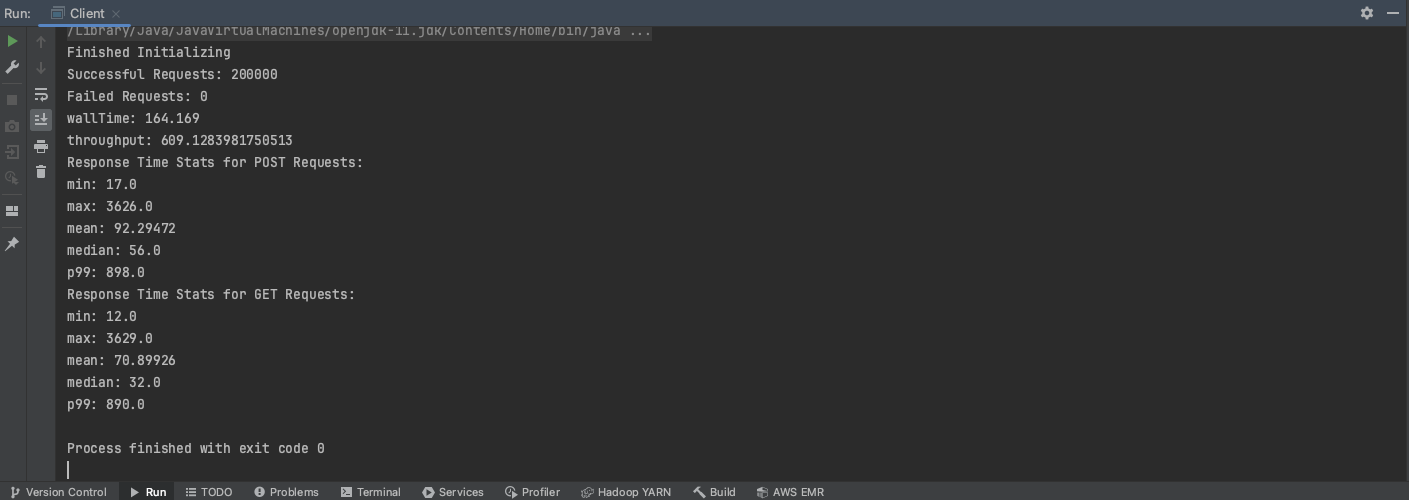
\includegraphics[width=\textwidth]{images/single_servlet_10.png}
    \caption{Single Servlet - threadGroupSize = 10, numThreadGroups = 10, delay = 2}
\end{figure}
\begin{figure}[H]
    \centering
    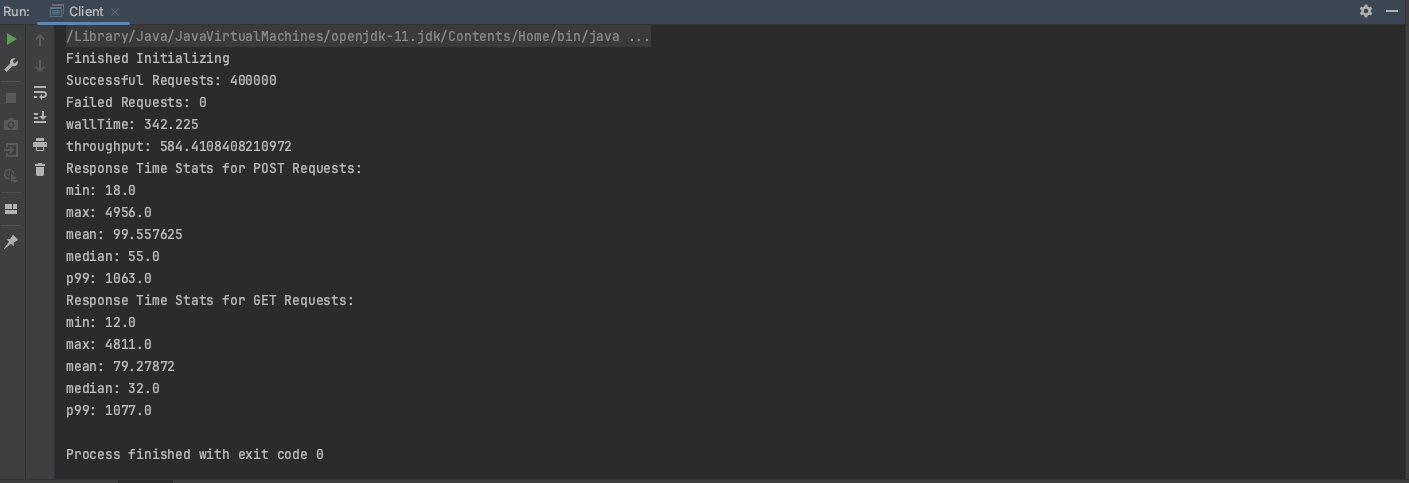
\includegraphics[width=\textwidth]{images/single_servlet_20.png}
    \caption{Single Servlet - threadGroupSize = 10, numThreadGroups = 20, delay = 2}
\end{figure}
\begin{figure}[H]
    \centering
    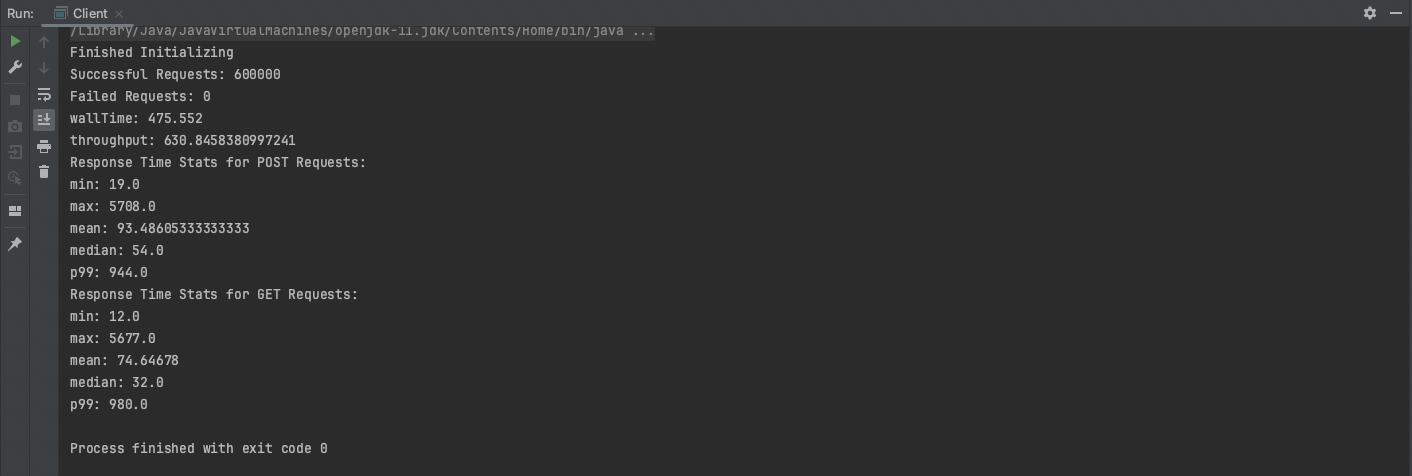
\includegraphics[width=\textwidth]{images/single_servlet_30.png}
    \caption{Single Servlet - threadGroupSize = 10, numThreadGroups = 30, delay = 2}
\end{figure}


\begin{table}[H]
    \centering
    \begin{tabular}{ccccc}
    \hline
    \multicolumn{2}{|c|}{}                                                      & \multicolumn{3}{c|}{Single Servlet}                                                         \\ \hline
    \multicolumn{2}{|c|}{Configuration}                                       & \multicolumn{1}{c|}{10/10/2} & \multicolumn{1}{c|}{10/20/2} & \multicolumn{1}{c|}{10/30/2} \\ \hline
    \multicolumn{2}{|c|}{Wall Time}                                           & \multicolumn{1}{c|}{164}     & \multicolumn{1}{c|}{342}     & \multicolumn{1}{c|}{476}     \\ \hline
    \multicolumn{2}{|c|}{Throughput}                                          & \multicolumn{1}{c|}{609}     & \multicolumn{1}{c|}{584}     & \multicolumn{1}{c|}{631}     \\ \hline
    \multicolumn{1}{|c|}{\multirow{5}{*}{Post}} & \multicolumn{1}{c|}{Min}    & \multicolumn{1}{c|}{17}      & \multicolumn{1}{c|}{18}      & \multicolumn{1}{c|}{19}      \\ \cline{2-5} 
    \multicolumn{1}{|c|}{}                      & \multicolumn{1}{c|}{Max}    & \multicolumn{1}{c|}{3626}    & \multicolumn{1}{c|}{4956}    & \multicolumn{1}{c|}{5708}    \\ \cline{2-5} 
    \multicolumn{1}{|c|}{}                      & \multicolumn{1}{c|}{Mean}   & \multicolumn{1}{c|}{92}      & \multicolumn{1}{c|}{100}     & \multicolumn{1}{c|}{93}      \\ \cline{2-5} 
    \multicolumn{1}{|c|}{}                      & \multicolumn{1}{c|}{Median} & \multicolumn{1}{c|}{56}      & \multicolumn{1}{c|}{55}      & \multicolumn{1}{c|}{54}      \\ \cline{2-5} 
    \multicolumn{1}{|c|}{}                      & \multicolumn{1}{c|}{P99}    & \multicolumn{1}{c|}{898}     & \multicolumn{1}{c|}{1063}    & \multicolumn{1}{c|}{944}     \\ \hline
    \multicolumn{1}{|c|}{\multirow{5}{*}{Get}}  & \multicolumn{1}{c|}{Min}    & \multicolumn{1}{c|}{12}      & \multicolumn{1}{c|}{12}      & \multicolumn{1}{c|}{12}      \\ \cline{2-5} 
    \multicolumn{1}{|c|}{}                      & \multicolumn{1}{c|}{Max}    & \multicolumn{1}{c|}{3629}    & \multicolumn{1}{c|}{4811}    & \multicolumn{1}{c|}{5677}    \\ \cline{2-5} 
    \multicolumn{1}{|c|}{}                      & \multicolumn{1}{c|}{Mean}   & \multicolumn{1}{c|}{71}      & \multicolumn{1}{c|}{79}      & \multicolumn{1}{c|}{75}      \\ \cline{2-5} 
    \multicolumn{1}{|c|}{}                      & \multicolumn{1}{c|}{Median} & \multicolumn{1}{c|}{32}      & \multicolumn{1}{c|}{32}      & \multicolumn{1}{c|}{32}      \\ \cline{2-5} 
    \multicolumn{1}{|c|}{}                      & \multicolumn{1}{c|}{P99}    & \multicolumn{1}{c|}{890}     & \multicolumn{1}{c|}{1077}    & \multicolumn{1}{c|}{980}      \\ \hline
    \end{tabular}
    \caption{Statistics for single servlet}
\end{table}


\newpage
\item {\it Output windows for the 3 client configuration tests run against a two load balanced servers/DB (15 points)}

\begin{figure}[H]
    \centering
    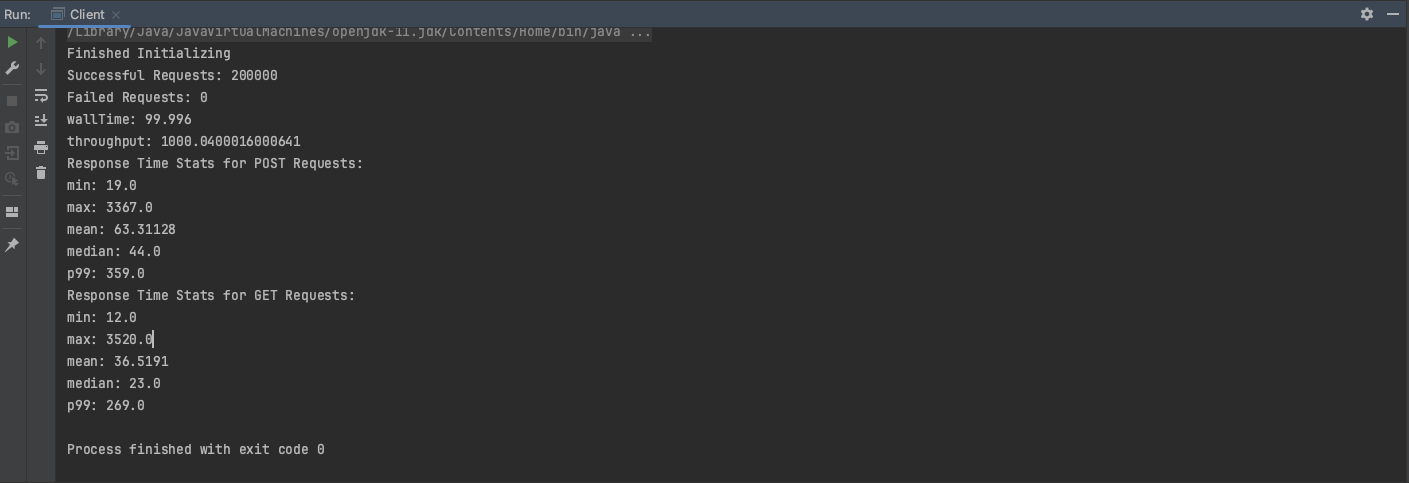
\includegraphics[width=\textwidth]{images/two_servlet_10.png}
    \caption{Two Load Balanced Servlet - threadGroupSize = 10, numThreadGroups = 10, delay = 2}
\end{figure}
\begin{figure}[H]
    \centering
    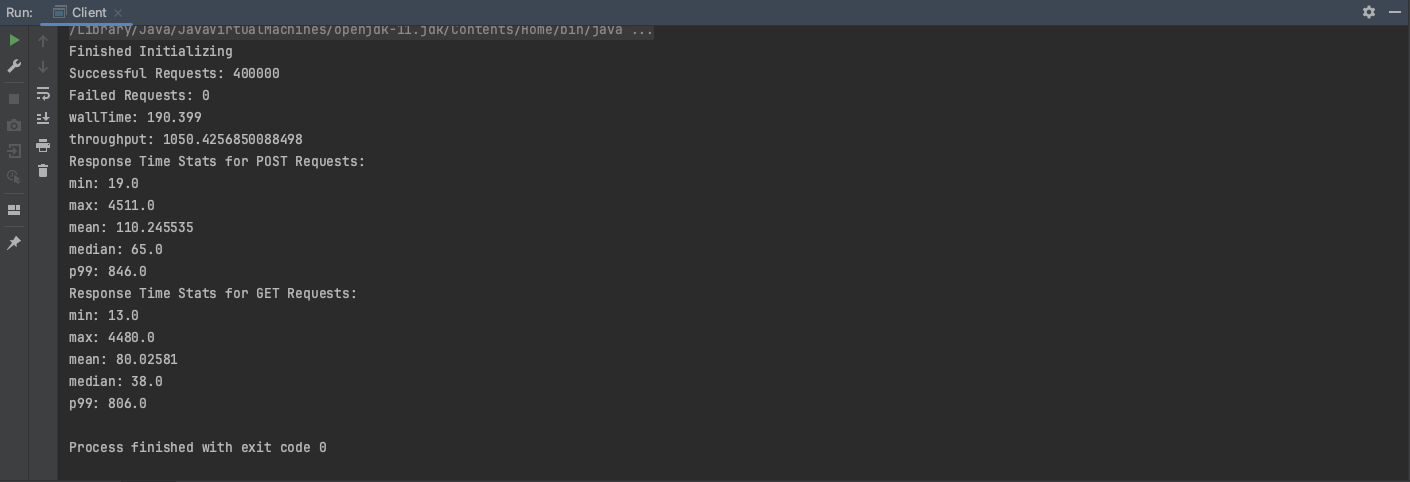
\includegraphics[width=\textwidth]{images/two_servlet_20.png}
    \caption{Two Load Balanced Servlet - threadGroupSize = 10, numThreadGroups = 20, delay = 2}
\end{figure}
\begin{figure}[H]
    \centering
    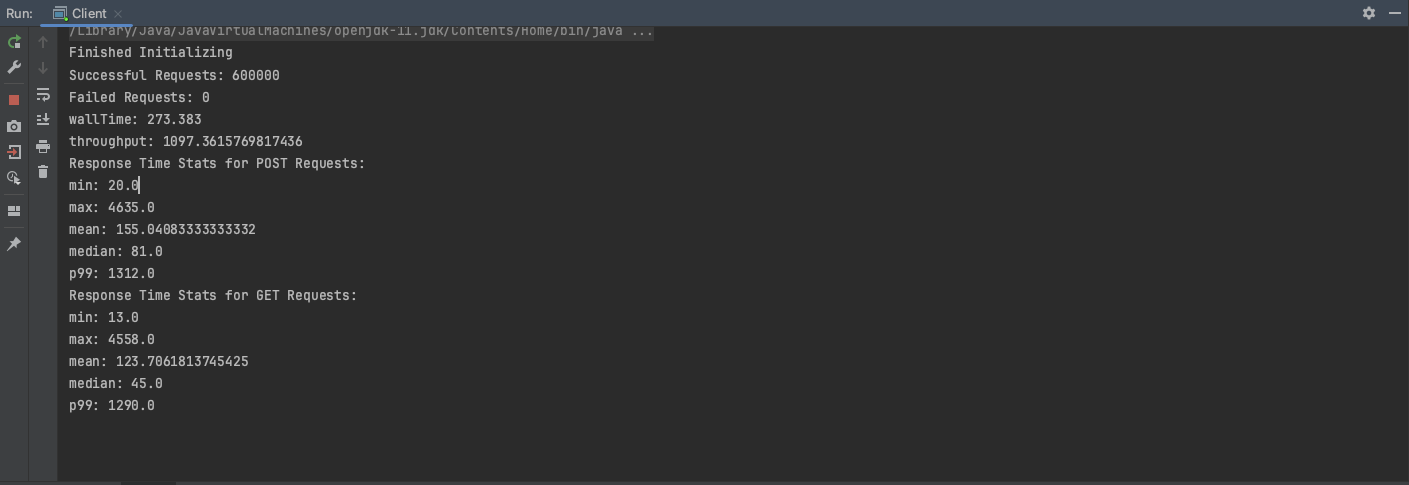
\includegraphics[width=\textwidth]{images/two_server_30.png}
    \caption{Two Load Balanced Servlet - threadGroupSize = 10, numThreadGroups = 30, delay = 2}
\end{figure}

\begin{table}[H]
    \centering
    \begin{tabular}{|cc|ccc|}
    \hline
    \multicolumn{2}{|c|}{}                               & \multicolumn{3}{c|}{Two Load Balanced Servlets}                       \\ \hline
    \multicolumn{2}{|c|}{Configuration}                  & \multicolumn{1}{c|}{10/10/2} & \multicolumn{1}{c|}{10/20/2} & 10/30/2 \\ \hline
    \multicolumn{2}{|c|}{Wall Time}                      & \multicolumn{1}{c|}{100}     & \multicolumn{1}{c|}{190}     & 273     \\ \hline
    \multicolumn{2}{|c|}{Throughput}                     & \multicolumn{1}{c|}{1000}    & \multicolumn{1}{c|}{1050}    & 1097    \\ \hline
    \multicolumn{1}{|c|}{\multirow{5}{*}{Post}} & Min    & \multicolumn{1}{c|}{19}      & \multicolumn{1}{c|}{19}      & 20      \\ \cline{2-5} 
    \multicolumn{1}{|c|}{}                      & Max    & \multicolumn{1}{c|}{3367}    & \multicolumn{1}{c|}{4511}    & 4635    \\ \cline{2-5} 
    \multicolumn{1}{|c|}{}                      & Mean   & \multicolumn{1}{c|}{63}      & \multicolumn{1}{c|}{110}     & 155     \\ \cline{2-5} 
    \multicolumn{1}{|c|}{}                      & Median & \multicolumn{1}{c|}{44}      & \multicolumn{1}{c|}{65}      & 81      \\ \cline{2-5} 
    \multicolumn{1}{|c|}{}                      & P99    & \multicolumn{1}{c|}{359}     & \multicolumn{1}{c|}{846}     & 1312    \\ \hline
    \multicolumn{1}{|c|}{\multirow{5}{*}{Get}}  & Min    & \multicolumn{1}{c|}{12}      & \multicolumn{1}{c|}{13}      & 13      \\ \cline{2-5} 
    \multicolumn{1}{|c|}{}                      & Max    & \multicolumn{1}{c|}{3520}    & \multicolumn{1}{c|}{4480}    & 4558    \\ \cline{2-5} 
    \multicolumn{1}{|c|}{}                      & Mean   & \multicolumn{1}{c|}{37}      & \multicolumn{1}{c|}{80}      & 124     \\ \cline{2-5} 
    \multicolumn{1}{|c|}{}                      & Median & \multicolumn{1}{c|}{23}      & \multicolumn{1}{c|}{38}      & 45      \\ \cline{2-5} 
    \multicolumn{1}{|c|}{}                      & P99    & \multicolumn{1}{c|}{269}     & \multicolumn{1}{c|}{806}     & 1290    \\ \hline
    \end{tabular}
    \caption{Statistics for two load balanced servers}
    \end{table}
\newpage
\item  {\it Output window for optimized server configuration for client with 30 Thread Groups. Briefly describe what configuration changes you made and what \% throughput improvement you achieved (15 points)}

\begin{figure}[H]
    \centering
    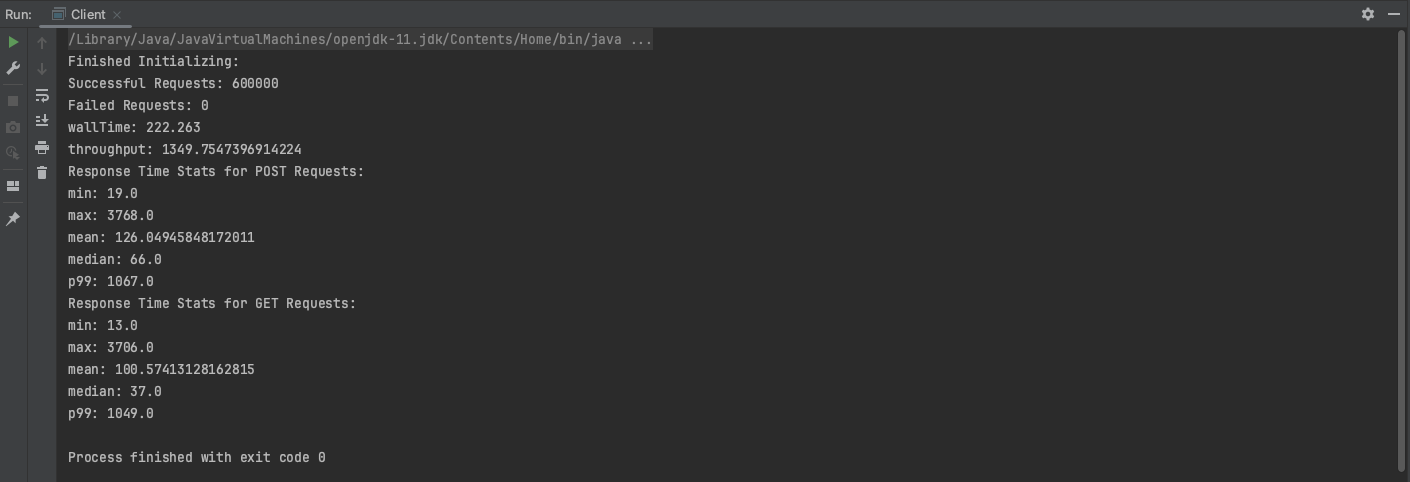
\includegraphics[width=\textwidth]{images/optimized_30.png}
    \caption{Optimized Load Balanced Servlets - threadGroupSize = 10, numThreadGroups = 30, delay = 2}
\end{figure}

\begin{table}[H]
    \centering
    \begin{tabular}{|cc|c|}
    \hline
    \multicolumn{2}{|c|}{}                               & Optimized Servlets \\ \hline
    \multicolumn{2}{|c|}{Configuration}                  & 10/30/2            \\ \hline
    \multicolumn{2}{|c|}{Wall Time}                      & 222.263            \\ \hline
    \multicolumn{2}{|c|}{Throughput}                     & 1350               \\ \hline
    \multicolumn{1}{|c|}{\multirow{5}{*}{Post}} & Min    & 19                 \\ \cline{2-3} 
    \multicolumn{1}{|c|}{}                      & Max    & 3768               \\ \cline{2-3} 
    \multicolumn{1}{|c|}{}                      & Mean   & 126                \\ \cline{2-3} 
    \multicolumn{1}{|c|}{}                      & Median & 66                 \\ \cline{2-3} 
    \multicolumn{1}{|c|}{}                      & P99    & 1067               \\ \hline
    \multicolumn{1}{|c|}{\multirow{5}{*}{Get}}  & Min    & 13                 \\ \cline{2-3} 
    \multicolumn{1}{|c|}{}                      & Max    & 3706               \\ \cline{2-3} 
    \multicolumn{1}{|c|}{}                      & Mean   & 101                \\ \cline{2-3} 
    \multicolumn{1}{|c|}{}                      & Median & 37                 \\ \cline{2-3} 
    \multicolumn{1}{|c|}{}                      & P99    & 1049               \\ \hline
    \end{tabular}
    \caption{Statistics for Optimized Servlets}
\end{table}

After analyzing the graphs shown in the monitoring tools of AWS, I found out that the cpu utilization
for one of the instance reached 61\% and the other reached 73\%. Although the utilization is high, 
they never reached above 75\% so I do not believe the servlets to be the bottleneck. Then I checked the
rds instance and found out that the maximum concurrent connections established to be 84 connections, which
is close to the maximum of 90 connections as I set for the connection pool. On the other hand, the cpu utilization
for the rds instance reached 87\%.

\begin{figure}[H]
    \begin{subfigure}{.475\linewidth}
        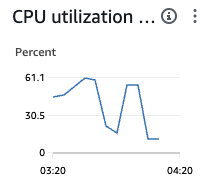
\includegraphics[width=\linewidth]{images/instance1_util.png}
        \caption{CPU Utilization for 1st Instance}
        \label{MLEDdet}
    \end{subfigure}\hfill % <-- "\hfill"
    \begin{subfigure}{.475\linewidth}
        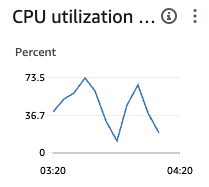
\includegraphics[width=\linewidth]{images/instance2_util.png}
        \caption{CPU Utilization for 2nd Instance}
        \label{energydetPSK}
    \end{subfigure}
    
    \medskip % create some *vertical* separation between the graphs
    \begin{subfigure}{.475\linewidth}
        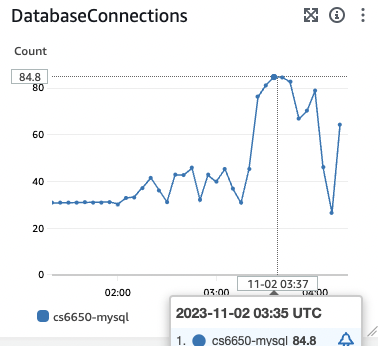
\includegraphics[width=\linewidth]{images/db_connections.png}
        \caption{RDS Connection Count}
        \label{velcomp}
    \end{subfigure}\hfill % <-- "\hfill"
    \begin{subfigure}{.475\linewidth}
        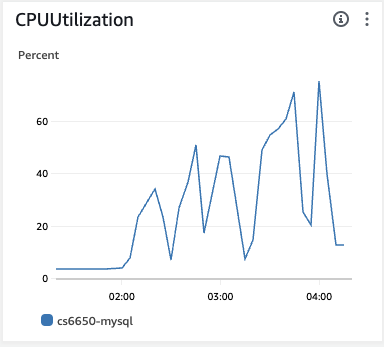
\includegraphics[width=\linewidth]{images/db_cpu_utilization.png}
        \caption{CPU Utilization for RDS Instance}
        \label{estcomp}
    \end{subfigure}
    
    \caption{A figure with four subfigures}
    \label{fig:roc}
\end{figure}
  

Therefore I changed the instance type from the free tier db.t3.micro to db.t3.small. The results show that there
was about 23\% in the throughput.

\begin{table}[H]
    \centering
    \begin{tabular}{|cc|ccc|ccc|c|}
    \hline
    \multicolumn{2}{|c|}{}                               & \multicolumn{3}{c|}{Single Servlet}                                   & \multicolumn{3}{c|}{Two Load Balanced Servlets}                       & Optimized Servlets \\ \hline
    \multicolumn{2}{|c|}{Configuration}                  & \multicolumn{1}{c|}{10/10/2} & \multicolumn{1}{c|}{10/20/2} & 10/30/2 & \multicolumn{1}{c|}{10/10/2} & \multicolumn{1}{c|}{10/20/2} & 10/30/2 & 10/30/2            \\ \hline
    \multicolumn{2}{|c|}{Wall Time}                      & \multicolumn{1}{c|}{164}     & \multicolumn{1}{c|}{342}     & 476     & \multicolumn{1}{c|}{100}     & \multicolumn{1}{c|}{190}     & 273     & 222.263            \\ \hline
    \multicolumn{2}{|c|}{Throughput}                     & \multicolumn{1}{c|}{609}     & \multicolumn{1}{c|}{584}     & 631     & \multicolumn{1}{c|}{1000}    & \multicolumn{1}{c|}{1050}    & 1097    & 1350               \\ \hline
    \multicolumn{1}{|c|}{\multirow{5}{*}{Post}} & Min    & \multicolumn{1}{c|}{17}      & \multicolumn{1}{c|}{18}      & 19      & \multicolumn{1}{c|}{19}      & \multicolumn{1}{c|}{19}      & 20      & 19                 \\ \cline{2-9} 
    \multicolumn{1}{|c|}{}                      & Max    & \multicolumn{1}{c|}{3626}    & \multicolumn{1}{c|}{4956}    & 5708    & \multicolumn{1}{c|}{3367}    & \multicolumn{1}{c|}{4511}    & 4635    & 3768               \\ \cline{2-9} 
    \multicolumn{1}{|c|}{}                      & Mean   & \multicolumn{1}{c|}{92}      & \multicolumn{1}{c|}{100}     & 93      & \multicolumn{1}{c|}{63}      & \multicolumn{1}{c|}{110}     & 155     & 126                \\ \cline{2-9} 
    \multicolumn{1}{|c|}{}                      & Median & \multicolumn{1}{c|}{56}      & \multicolumn{1}{c|}{55}      & 54      & \multicolumn{1}{c|}{44}      & \multicolumn{1}{c|}{65}      & 81      & 66                 \\ \cline{2-9} 
    \multicolumn{1}{|c|}{}                      & P99    & \multicolumn{1}{c|}{898}     & \multicolumn{1}{c|}{1063}    & 944     & \multicolumn{1}{c|}{359}     & \multicolumn{1}{c|}{846}     & 1312    & 1067               \\ \hline
    \multicolumn{1}{|c|}{\multirow{5}{*}{Get}}  & Min    & \multicolumn{1}{c|}{12}      & \multicolumn{1}{c|}{12}      & 12      & \multicolumn{1}{c|}{12}      & \multicolumn{1}{c|}{13}      & 13      & 13                 \\ \cline{2-9} 
    \multicolumn{1}{|c|}{}                      & Max    & \multicolumn{1}{c|}{3629}    & \multicolumn{1}{c|}{4811}    & 5677    & \multicolumn{1}{c|}{3520}    & \multicolumn{1}{c|}{4480}    & 4558    & 3706               \\ \cline{2-9} 
    \multicolumn{1}{|c|}{}                      & Mean   & \multicolumn{1}{c|}{71}      & \multicolumn{1}{c|}{79}      & 75      & \multicolumn{1}{c|}{37}      & \multicolumn{1}{c|}{80}      & 124     & 101                \\ \cline{2-9} 
    \multicolumn{1}{|c|}{}                      & Median & \multicolumn{1}{c|}{32}      & \multicolumn{1}{c|}{32}      & 32      & \multicolumn{1}{c|}{23}      & \multicolumn{1}{c|}{38}      & 45      & 37                 \\ \cline{2-9} 
    \multicolumn{1}{|c|}{}                      & P99    & \multicolumn{1}{c|}{890}     & \multicolumn{1}{c|}{1077}    & 980     & \multicolumn{1}{c|}{269}     & \multicolumn{1}{c|}{806}     & 1290    & 1049               \\ \hline
    \end{tabular}
    \caption{Statistics for all runs}
    \end{table}

\end{enumerate}

\clearpage

\end{document}
